\documentclass[oneside,a4paper]{book}
\usepackage{vpcpc}
\usepackage[utf8]{inputenc}
\usepackage{ksp-lst-utf8}  % makra na listingy programov

\usepackage[absolute]{textpos}
\setlength{\TPHorizModule}{1cm}
\setlength{\TPVertModule}{\TPHorizModule}
\textblockorigin{0cm}{0cm}

\begin{document}
\mainmatter
\thispagestyle{empty}
{~}
\vspace{1cm}
\noindent
\centerline{\scalebox{4.0}{\huge\sf\bfseries VPCPC 2014~}}
\vspace{0.7cm}
\centerline{\scalebox{1.4}{\huge\sf\bfseries problems and sample solutions}}

\vfill

\begin{textblock}{10}(2,10)
\noindent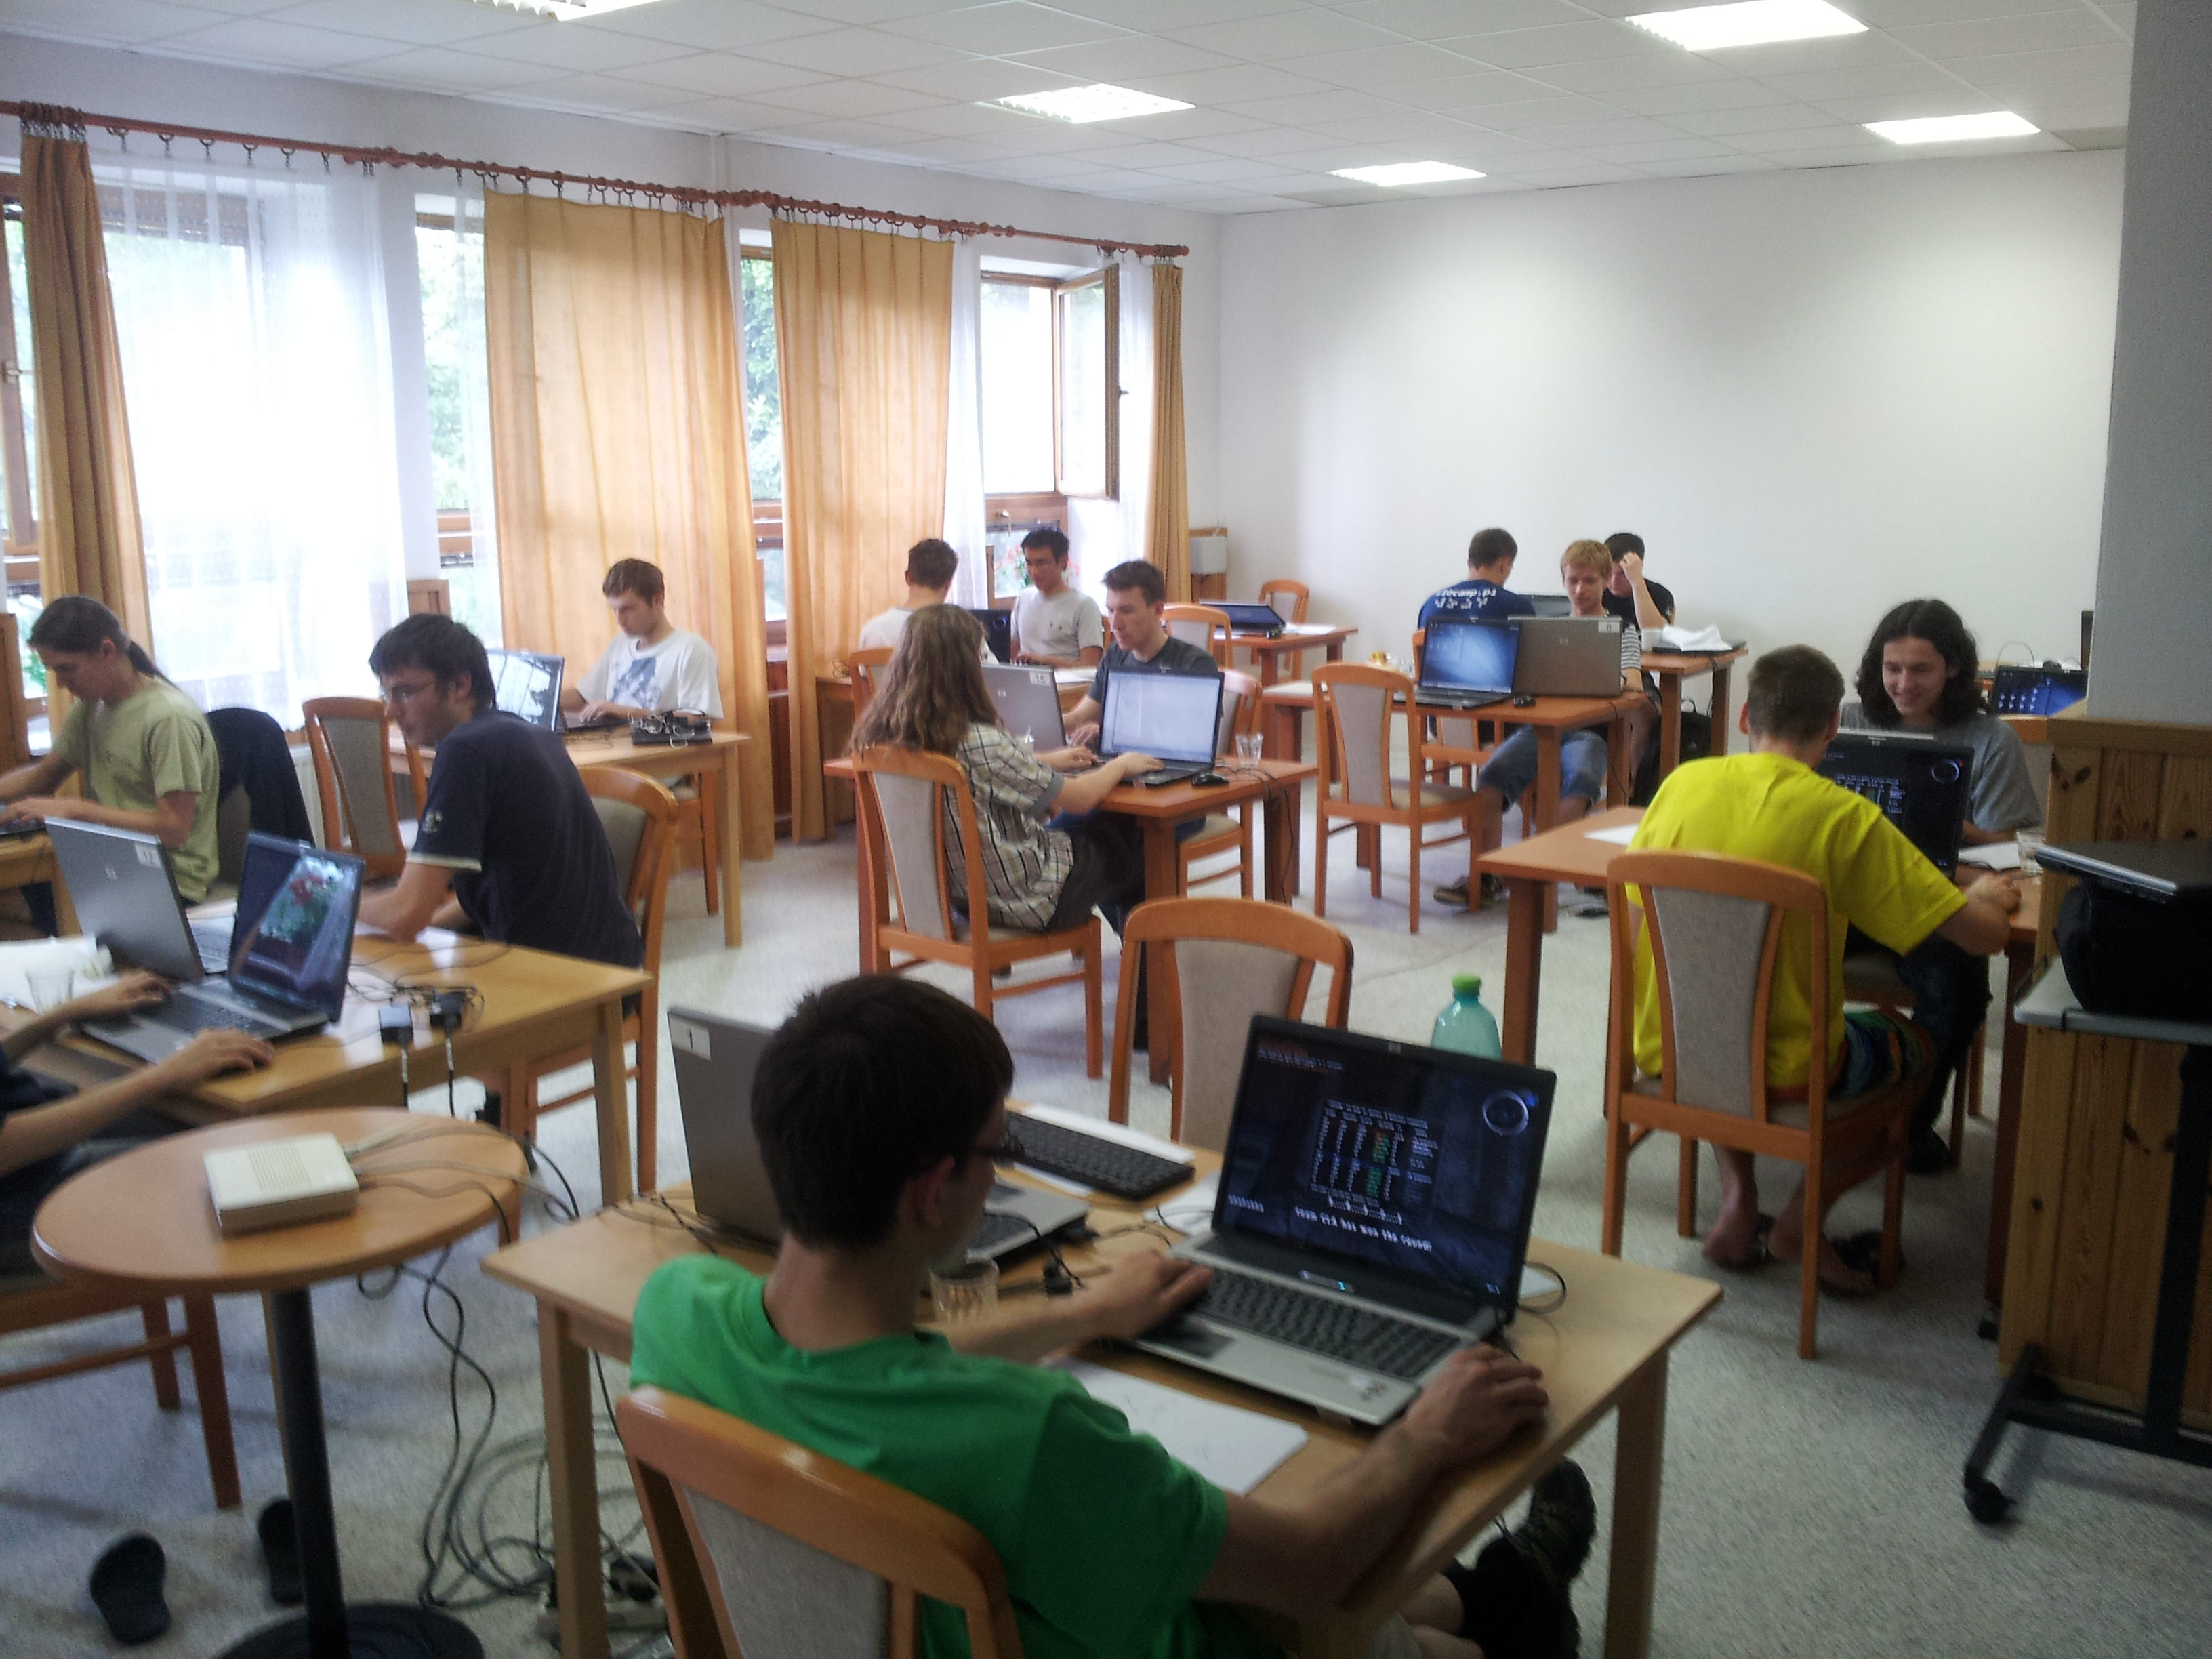
\includegraphics[height=7cm]{photos/coding.jpg}
\end{textblock}

\begin{textblock}{14}(6,16)
\noindent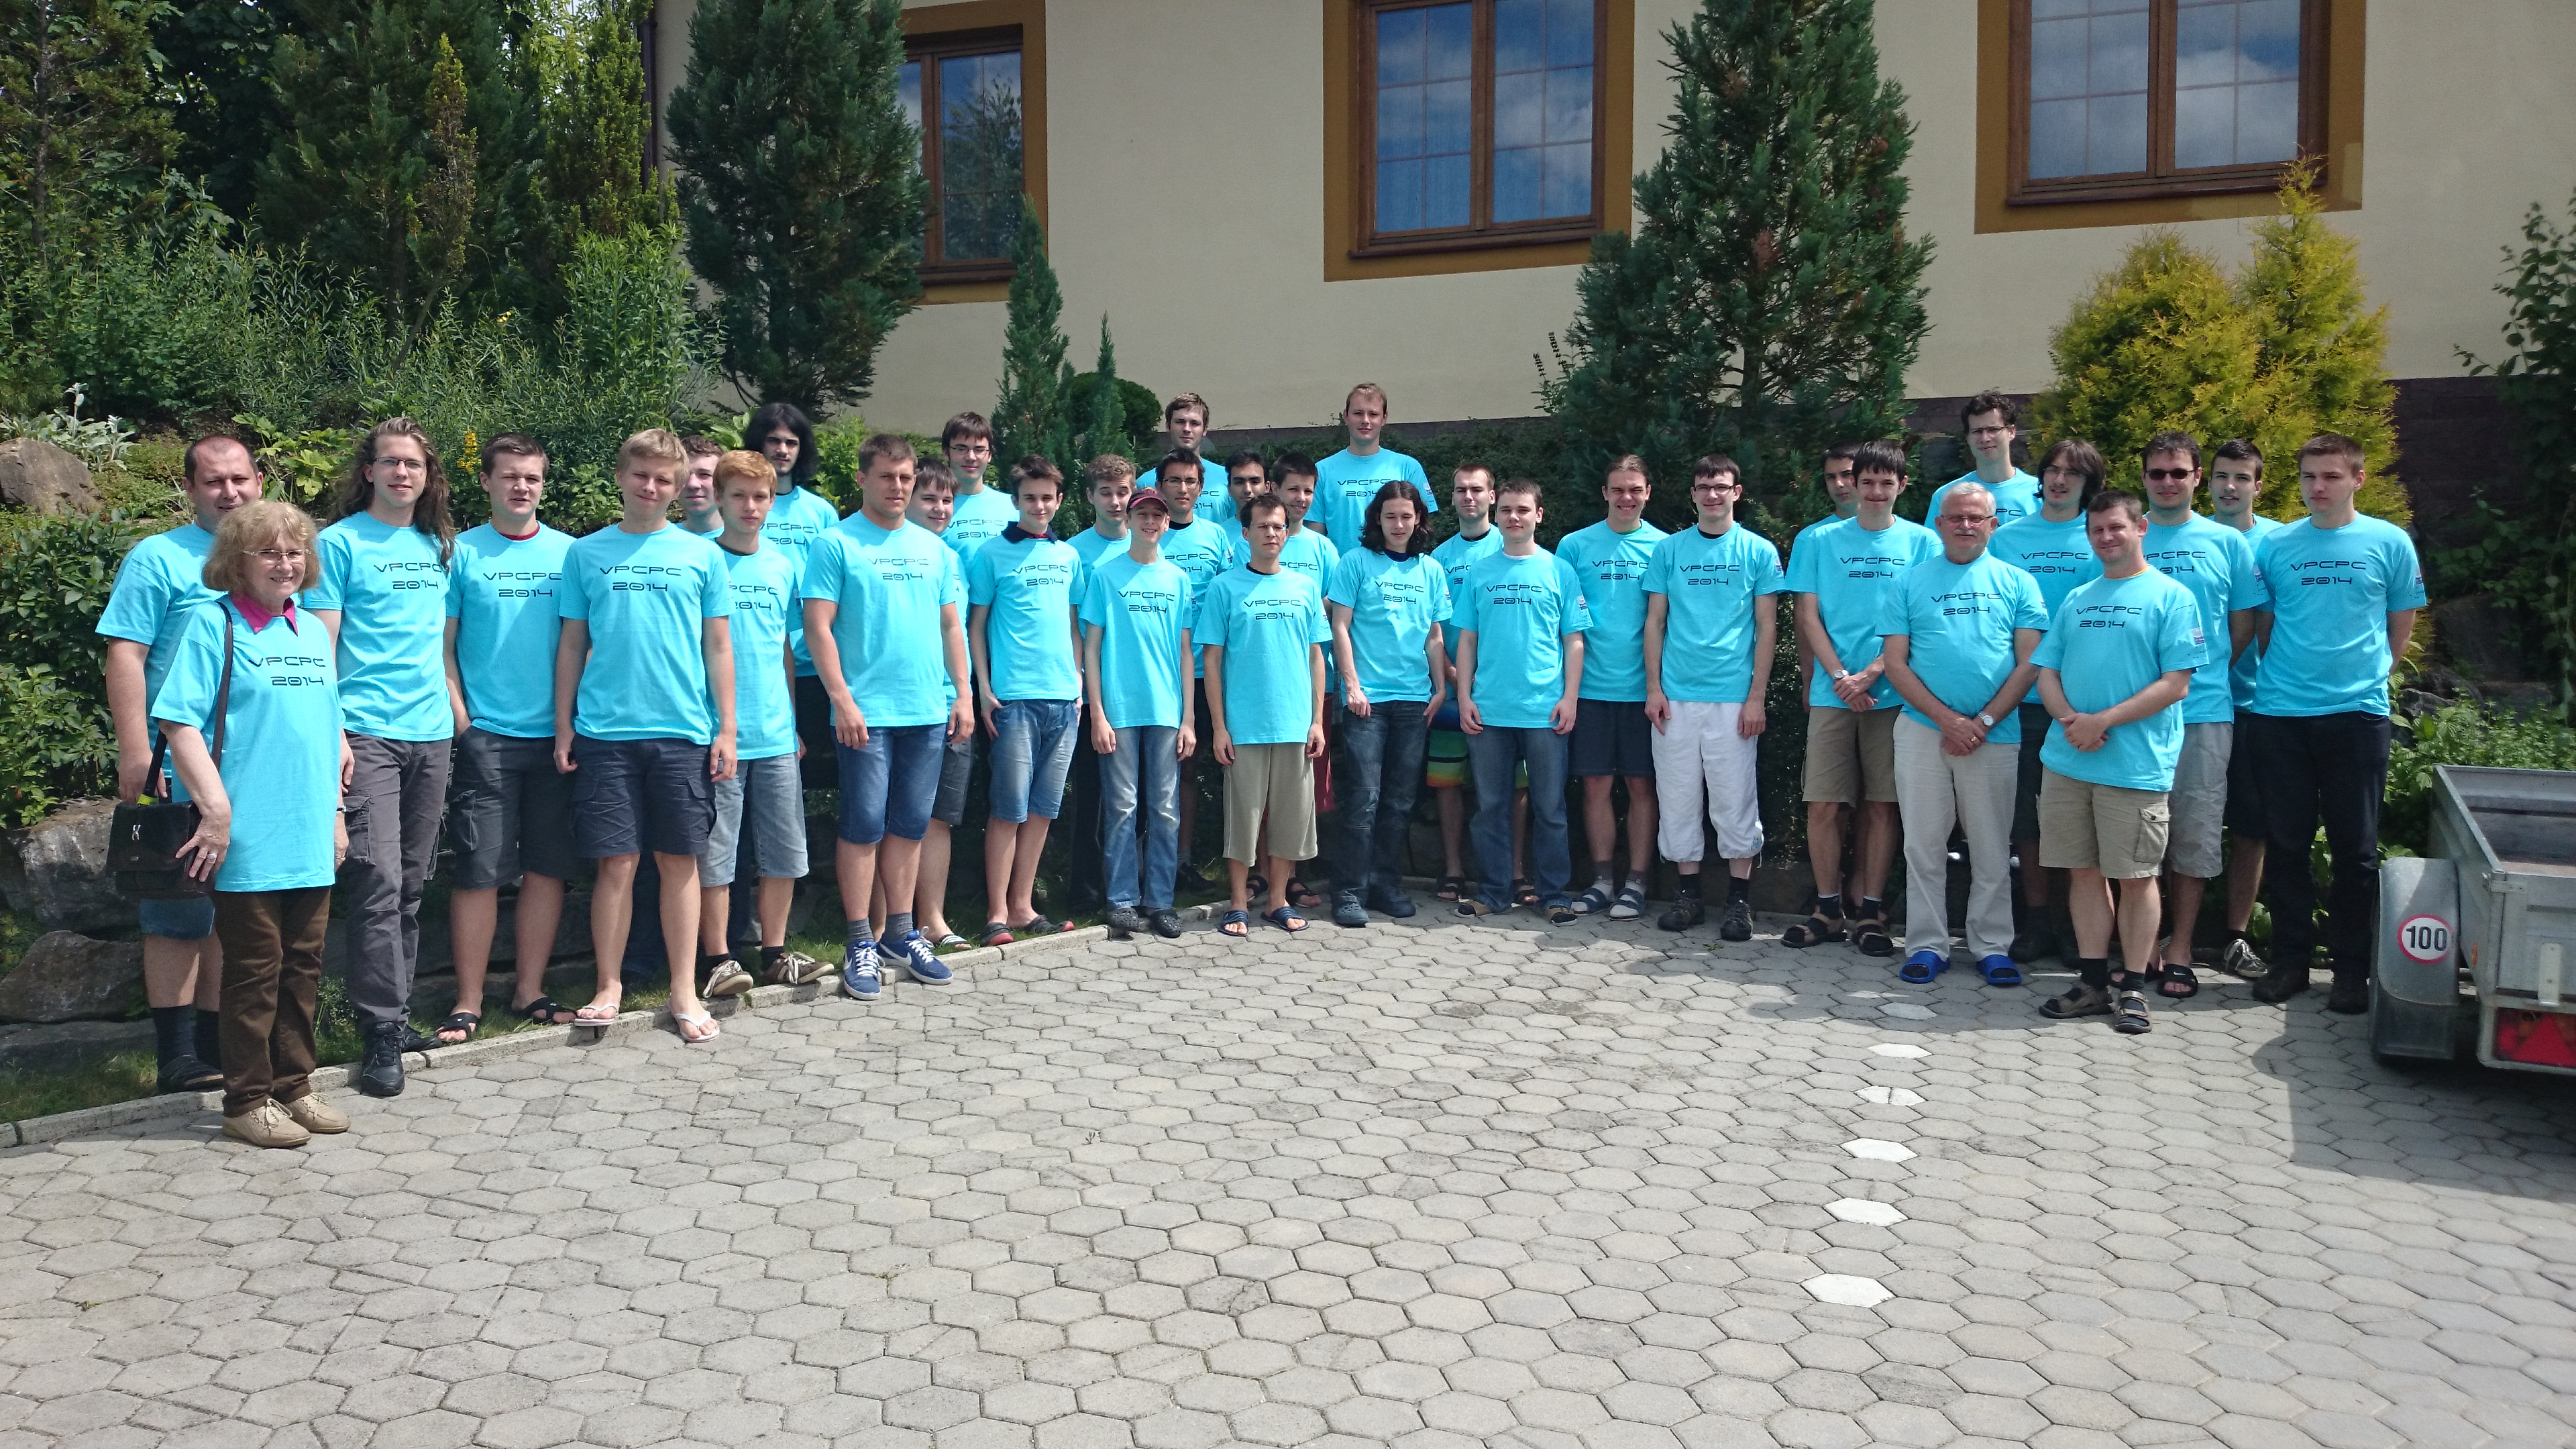
\includegraphics[height=7cm]{photos/tshirts.jpg}
\end{textblock}

\begin{textblock}{5}(12.5,11.5)
\noindent
\includegraphics[height=2.5cm]{img/vf_logo_v2.pdf}
\end{textblock}

The first ever Visegrad Programming Contests Preparation Camp took place in Danišovce, Slovakia,
between June 28th and July 6th, 2014. The camp was attended by delegations from all four Visegrad
countries: Czech Republic, Hungary, Poland, and Slovakia. The camp was partially supported
by the Visegrad Fund Small Grant 11340003.
\newpage

\noindent\centerline{\sf\Large\bfseries Table of Contents}
\makeatletter\let\l@section\l@chapter\let\l@chapter\l@part\@starttoc{toc}\makeatother
\newpage

\addtocontents{toc}{\par}
\addcontentsline{toc}{chapter}{Part 0: About the camp}
\refstepcounter{section}\addcontentsline{toc}{section}{Preface}
\noindent\centerline{\sf\large\bfseries Preface}
\bigskip

Hello, dear reader!
\bigskip

This booklet contains all tasks and solution writeups from the
first ever Visegrad Programming Contest Preparation Camp (VPCPC).
The VPCPC is continuing and extending a long tradition of 
international algorithmic preparation camps in central Europe.
The predecessor of this camp was the Czech-Polish-Slovak
Preparation Camp (CPSPC). This camp has been organized once per year
by one of the three participating countries. The first ever CPSPC
took place in the summer of 1999 in Belušské Slatiny, Slovakia.
After starting that tradition, we are now hoping that we were able
to start a new, even better one. We would love to see and attend
many more VPCPCs in the years to come!
\bigskip

Anyway, let's get back to the tasks. The participants invited to
the camp are secondary school students who are among the best in
algorithmic problem solving. Most of them are future participants
in the International Olympiad in Informatics (IOI) and similar
contests. The 20 tasks used at VPCPC 2014 reflect the skill level
of these contestants. (Read: most of the tasks are quite difficult.)
\bigskip

The test data for all the tasks is available at
\url{https://github.com/trojsten/vpcpc}.
All the materials from the camp are released under the
Creative Commons Attribution-ShareAlike (CC BY-SA) 3.0 
license.
\bigskip

\null\hfill Michal Forišek \\
\null\hfill Bratislava, July 2014

\newpage

\refstepcounter{section}\addcontentsline{toc}{section}{Results}
\noindent\centerline{\sf\large\bfseries Results}
\bigskip
\safeinput{results}
\newpage

\refstepcounter{section}\addcontentsline{toc}{section}{Statistics}
\noindent\centerline{\sf\large\bfseries Statistics}
\bigskip
\safeinput{stats}
\newpage

\addtocontents{toc}{\par}
\refstepcounter{chapter}\addcontentsline{toc}{chapter}{Part I: Problem statements}
\refstepcounter{section}\addcontentsline{toc}{section}{Day 1: Slovak problems}
\safeinput{statements/day1-hyperways}\newpage
\safeinput{statements/day1-malloc}\newpage
\safeinput{statements/day1-shades}\newpage

\phantomsection
\refstepcounter{section}\addcontentsline{toc}{section}{Day 2: Czech problems}
\safeinput{statements/day2-buslines}\newpage
\safeinput{statements/day2-cutting}\newpage
\safeinput{statements/day2-investigation}\newpage

\refstepcounter{section}\addcontentsline{toc}{section}{Day 3: Mixed problems}
\safeinput{statements/day3-newtree}\newpage
\safeinput{statements/day3-rubik}\newpage
\safeinput{statements/day3-universities}\newpage
\safeinput{statements/day3-wall}\newpage

\refstepcounter{section}\addcontentsline{toc}{section}{Day 4: Hungarian problems}
\safeinput{statements/day4-critical}\newpage
\safeinput{statements/day4-networks}\newpage
\safeinput{statements/day4-nextperm}\newpage

\refstepcounter{section}\addcontentsline{toc}{section}{Day 5: Polish problems}
\safeinput{statements/day5-game}\newpage
\safeinput{statements/day5-posters}\newpage
\safeinput{statements/day5-sorting}\newpage

\refstepcounter{section}\addcontentsline{toc}{section}{Day 6: Mixed problems}
\safeinput{statements/day6-mission}\newpage
\safeinput{statements/day6-newspapers}\newpage
\safeinput{statements/day6-slalom}\newpage
\safeinput{statements/day6-tickets}\newpage

\addtocontents{toc}{\par}
\refstepcounter{part}
\addcontentsline{toc}{chapter}{Part II: Solutions}
\refstepcounter{section}\addcontentsline{toc}{section}{Day 1: Slovak problems}
\safeinput{solutions/day1-hyperways}\newpage
\safeinput{solutions/day1-malloc}\newpage
\safeinput{solutions/day1-shades}\newpage

\phantomsection
\refstepcounter{section}\addcontentsline{toc}{section}{Day 2: Czech problems}
\safeinput{solutions/day2-buslines}\newpage
\safeinput{solutions/day2-cutting}\newpage
\safeinput{solutions/day2-investigation}\newpage

\refstepcounter{section}\addcontentsline{toc}{section}{Day 3: Mixed problems}
\safeinput{solutions/day3-newtree}\newpage
\safeinput{solutions/day3-rubik}\newpage
\safeinput{solutions/day3-universities}\newpage
\safeinput{solutions/day3-wall}\newpage

\refstepcounter{section}\addcontentsline{toc}{section}{Day 4: Hungarian problems}
\safeinput{solutions/day4-critical}\newpage
\safeinput{solutions/day4-networks}\newpage
\safeinput{solutions/day4-nextperm}\newpage

\refstepcounter{section}\addcontentsline{toc}{section}{Day 5: Polish problems}
\safeinput{solutions/day5-game}\newpage
\safeinput{solutions/day5-posters}\newpage
\safeinput{solutions/day5-sorting}\newpage

\refstepcounter{section}\addcontentsline{toc}{section}{Day 6: Mixed problems}
\safeinput{solutions/day6-mission}\newpage
\safeinput{solutions/day6-newspapers}\newpage
\safeinput{solutions/day6-slalom}\newpage
\safeinput{solutions/day6-tickets}\newpage

\end{document}
